\documentclass[tikz,border=2pt]{standalone}
\usepackage{tikz}
\usepackage{lmodern}
\usetikzlibrary{calc,decorations.pathreplacing}

% Visual conventions follow the existing MRNC TikZ pictures: ordinary
% components use TikZ's normal 0.4pt stroke, with compact TeX labels.
\tikzset{
  nu fibre/.style={
    x=0.78cm,
    y=0.78cm,
    line width=0.4pt,
    line cap=round,
    line join=round
  },
  nu label/.style={
    font=\scriptsize,
    inner sep=1pt
  },
  nu annotation/.style={
    font=\scriptsize,
    inner sep=1pt
  },
  nu dots/.style={
    font=\small,
    inner sep=0pt
  }
}

\begin{document}
% Namikawa--Ueno type VIII-1; NU p. 14.
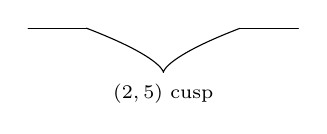
\begin{tikzpicture}[nu fibre]

  \draw[samples=140,smooth,domain=-1:1]
    plot ({1.25*(\x)^3},{-0.42+0.72*(\x)^2});
  \draw (-2.20,0.30) -- (-1.25,0.30);
  \draw (1.25,0.30) -- (2.20,0.30);
  \node[nu annotation,below=3pt] at (0,-0.42) {$(2,5)\ \mathrm{cusp}$};

\end{tikzpicture}
\end{document}
